\documentclass[10pt,a4paper]{article}
\usepackage[utf8]{inputenc}
\usepackage[czech]{babel}
\usepackage[T1]{fontenc}
\usepackage{graphicx}
\usepackage{amsmath}
\usepackage{ amssymb }
\usepackage{float}
\usepackage{fullpage}


\title{Teoretické základy informatiky}

\begin{document}
\maketitle



\newpage

\section{První odstavec}

Formální jazyky a jejich hierarchie. Regulární jazyky (definice, uzávěrové vlastnosti). Konečné automaty deterministické
a nedeterministické. Regulární výrazy, automaty s epsilon-přechody. Minimalizace konečného deterministického
automatu. Pumping lemma. Bezkontextové jazyky a jejich vlastnosti (uzávěrové vlastnosti, jednoznačnost).
Zásobníkové automaty a jejich modifikace. Deterministické zásobníkové automaty. Deterministické
bezkontextové jazyky.

%============================================================================
%                                                                             DRUHÝ ODSTAVEC
%============================================================================

\section{Druhý odstavec}

Turingův stroj (TS), nedeterministický TS. Jazyk přijímaný TS, jazyk rozhodovaný TS. Church-Turingova
teze, varianty TS. Částečně rekurzivní a rekurzivní jazyky, jazyky a rozhodovací problémy. Vztah rekurzivních
a částečně rekurzivních jazyků. Uzávěrové vlastnosti jazyků TS. Riceova věta. Vztah jazyků TS k jazykům
Chomského hierarchie. Věta o rekurzi.

	\subsection{Turingův stroj (TS)}

		\begin{itemize}
			\item Alan Turing, 1936
			\item účel: porozumět omezením mechanického výpočtu
		\end{itemize}
		\textbf{TS se skládá z}
		\begin{itemize}
			\item řídící jednotky, která se vždy nachází v jednom z konečného množství stavů
			\item zleva omezené nekonečné pásky rozdělené na políčka, v každém políčku je zapsán jeden symbol
			\item čtecí / zapisovací hlavy která je vždy umístěna nad jedním políčkem pásky
		\end{itemize}
		\textbf{Definice: }
		Turingův stroj je struktura $\langle Q, \Sigma, \Gamma, \delta, q_{start}, q_{+}, q_{-} \rangle $ dána:
		\begin{itemize}
			\item Neprázdnou konečnou množinou stavů $Q$
			\item Vstupní abecedou  $\Sigma$ t.ž. \textvisiblespace $ \notin \Sigma$
			\item páskovou abecedou $\Gamma$ t.ž. $\Sigma \subset \Gamma,$ \textvisiblespace $\in  \Gamma $
			\item přechodovou funkcí $\delta : Q \times  \Gamma \rightarrow Q \times \Gamma \times \{L , R \} $
			\item počátečním stavem $q_{start} \in Q$
			\item přijímacím stavem $q_{+} \in Q $ a zamítacím stavem $q_{-} \in Q.$ $q_{+} \neq q_{-}$
		\end{itemize}
		Program TS lze chápat jako množinu elementárních instrukcí ve tvaru:

		\textit{\uv{Pokud je řídící jednotka ve stavu $q$ a čtecí/zapisovací hlava čte symbol $a$, tak změň stav řídící jednotky
		na $q'$, na pásku zapiš $a'$ a posuň
		čtecí/zapisovací hlavu o jedno políčko směrem $d$.}}

		Takováto instrukce se zapisuje jako $\delta (q,a) = (q', a', d)$ a nazýváme ji přechod. Celý program, tedy množinu 				takovýchto instrukcí, pak nazýváme přechodovou funkcí TS

		\textbf{Konfigurace} TS je uspořádaná trojice $(q, \alpha, n) \in Q \times \Gamma^{*} \times N_{0}$ , která zachycuje
		aktuální status všech tří komponent.
		\begin{itemize}
			\item $q$ je aktuální stav řídící jednotky
			\item $\alpha$ je obsah pásky
			\item $n$ je pozice hlavy
		\end{itemize}

		\textbf{Krok výpočtu TS} je definován jako binární relace na množině konfigurací: Nechť $(q,a_{0} \dots a_{n}, i) $
		je taková konfigurace $T$, kde $q \neq q_{\pm}, n \in N_{0}, a_{0}, \dots, a_{n}~\in~\Gamma, i~\leq~n. $
		\begin{itemize}
			\item Je-li $1 \leq i \leq n a \delta(q,a_{i}) = (q', b, L), pak$
				$$(q,a_{0} \dots a_{n}, i) \vdash (q', a_{0} \dots a_{i-1}ba_{i+1} \dots a_{n}, i-1) $$
			\item Je-li $\delta(q,a_{0}) = (q', b, L), pak$
				$$(q,a_{0} \dots a_{n}, 0) \vdash (q', ba_{1} \dots a_{n}, 0) $$
			\item Je-li $\delta(q,a_{i}) = (q', b, R), pak$
				$$(q,a_{0} \dots a_{n}, i) \vdash (q', a_{0} \dots a_{i-1}ba_{i+1} \dots a_{n}, i+1) $$
		\end{itemize}



	\subsection{Nedeterministický TS}

		Obdobný rozdíl jako u konečných deterministických a konečných nedeterministických automatů. Přechodová funkce ve 				tvaru:
		$$\delta : Q \times  \Gamma \rightarrow 2^{Q \times \Gamma \times \{L , R \}}$$

		\textbf{Definice: }
		Nedeterministický TS je struktura $\langle Q, \Sigma, \Gamma, \delta, q_{start}, q_{+}, q_{-} \rangle $ dána:
		\begin{itemize}
			\item Neprázdnou konečnou množinou stavů $Q$
			\item Vstupní abecedou  $\Sigma$ t.ž. \textvisiblespace $ \notin \Sigma$
			\item páskovou abecedou $\Gamma$ t.ž. $\Sigma \subset \Gamma,$ \textvisiblespace $\in  \Gamma $
			\item přechodovou funkcí $\delta : Q \times  \Gamma \rightarrow 2^{Q \times \Gamma \times \{L , R \}} $
			\item počátečním stavem $q_{start} \in Q$
			\item přijímacím stavem $q_{+} \in Q $ a zamítacím stavem $q_{-} \in Q.$ $q_{+} \neq q_{-}$
		\end{itemize}

		Ke každému deterministickému existuje ekvivalentní nedeterministický automat a ke každému
		nedeterministickému existuje ekvivalentní deterministický automat.

	\subsection{Jazyk přijímaný TS}

		Množinu všech slov $\omega \in \Sigma^{*}$, které TS \textit{T} Přijímá značíme \textit{L(T)} a nazýváme 					\textit{\textbf{jazykem Turingova stroje}}, t.j.
		 $$L(T) = \{ \omega | \omega \in \Sigma^{*}, (\omega, q_{0},0) \vdash^{*} C_{+}\} $$
		Jazyk $L(T)$ nazýváme \textit{jazyk přijímaný TS} $T$.\\
		Říkáme, že TS $T$ \textit{přijímá jazyk}$ L(T)$.\\

		Jazyk $L \subseteq \Sigma^{*} $ nazveme\textit{ jazyk přijímaný TS}, pokud existuje TS $T$ který jej přijímá.

	\subsection{Jazyk rozhodovaný TS}

		Pokud navíc platí, že TS $T$ zamítá každé $\omega \notin L(T)$, nazýváme jazyk L(T)
		\textit{jazyk~rozhodovaný} TS $T$.\\
		Říkáme, že TS $T$ \textit{rozhoduje jazyk} $L(T)$. (to znamená že nikdy necyklí)

		Jazyk $L \subseteq \Sigma^{*} $ nazveme\textit{ jazyk rozhodovaný TS}, pokud existuje TS $T$ který jej rozhoduje.


	\subsection{Churg-Turingova teze}

		\textit{Intuitivní pojem algoritmu = algoritmus TS.} \\(to je všechno co k tomu máme)

	\subsection{Varianty TS}
		\begin{itemize}
			\item TS, který se nikdy nepokusí přejet levý okraj pásky
				\begin{itemize}
					\item Rozumíme TS, u kterého při výpočtu nad jakým koli slovem nedojde k tomu že, je v konfiguraci
						$(q,a\omega,0)$ a existuje přechod $\delta(q,a) = (q',b,L).$  Tedy nikdy nenastane situace
						že by byla hlava nad nejlevějším políčkem pásky a přechodová funkce by určovala pohyb 								vlevo.
				\end{itemize}
			\item TS, který nikdy nezapíše na pásku \textvisiblespace
				\begin{itemize}
					\item Roziníme TS, který nemá žádný přechod ve tvaru $\delta(q,a) = (q',\textvisiblespace,D)$
				\end{itemize}
			\item TS, který po sobě \uv{který po sobě uklízí}
				\begin{itemize}
					\item Roziníme TS, který zastaví pouze v konfiguraci $\langle q_{+}, \epsilon, 0 \rangle$
						nebo $\langle q_{-}, \epsilon, 0 \rangle$. Tzn. smaže obsah pásky.
				\end{itemize}
			\item ( předchozí 3 se nejspíš nepočítají mezi varianty TS)
			\item \textbf{TS s instrukcí stop} --- struktura  $\langle Q, \Sigma, \Gamma, \delta, q_{start}, q_{+}, q_{-} \rangle $
								dána:
				\begin{itemize}
					\item Neprázdnou konečnou množinou stavů $Q$
					\item Vstupní abecedou  $\Sigma$ t.ž. \textvisiblespace $ \notin \Sigma$
					\item páskovou abecedou $\Gamma$ t.ž. $\Sigma \subset \Gamma,$ \textvisiblespace $\in  \Gamma $
					\item přechodovou funkcí $\delta : Q \times  \Gamma \rightarrow Q \times \Gamma \times \{L, S, R \} $
					\item počátečním stavem $q_{start} \in Q$
					\item přijímacím stavem $q_{+} \in Q $ a zamítacím stavem $q_{-} \in Q.$ $q_{+} \neq q_{-}$
				\end{itemize}
				Odpovídajícím způsobem se upraví definice kroku výpočtu, vlatně se přidá bod:

				-- Je-li $\delta(q, a_{i}) = (q', b, S)$, pak
					$$(q,a_{0} \dots a_{n}, i) \vdash (q', a_{0} \dots a_{i-1}ba_{i+1} \dots a_{n},i) $$
			\item \textbf{TS s oboustranně nekonečnou páskou} --- definice je totožná jako u klasického TS; rozdíl je v definici
			 konfigurace (nevystačíme si s $\langle q, \omega, i \rangle \in Q \times \Gamma^{*} \times N_{0}$)a výpočtu
			(není zarážení o levý okraj)
				\begin{itemize}
					\item \textbf{Konfigurace:} Alternativně zapisujeme jako řetězec
					 	$\alpha q\beta \in \Gamma^{*}Q\Gamma^{*}.$
						Konfigurace $\alpha q\beta$ představuje status stroje, který má na pásce zapsán řetězec
						$ \alpha\beta$,
						hlava	je nad prvním symbolem řetězce $\beta$, řídící jednotka je ve stavu q.

						U TS s oboustranně nekonečnou páskou považujeme $\alpha q\beta$ za totožnou s
						$\alpha q\beta$\textvisiblespace a s \textvisiblespace$\alpha q\beta$.
					\item \textbf{Krok výpočtu TS (s oboustranně nekonečnou páskou)} je definován jako binární
						relace na množině konfigurací: Nechť $\alpha aqB\beta$ je taková konfigurace $T$, kde
						$q \neq q, \alpha, \beta \in \Gamma^{*}, a,b \in \Gamma.$
						\begin{itemize}
							\item Je-li $\delta(q,a) = (q', x, L) $, pak  $$\alpha aqb\beta \vdash \alpha q'ax\beta$$.
							\item Je-li $\delta(q,a_{1}) = (q', x, R) $, pak
									$$\alpha aqb\beta \vdash \alpha axq'\beta$$.
						\end{itemize}
				\end{itemize}
					\item \textbf{TS s více páskami} --- je struktura $\langle Q, \Sigma, \Gamma, \delta, q_{0}, q_{+},
						q_{-} \rangle $ dána:
						\begin{itemize}
							\item Neprázdnou konečnou množinou stavů $Q$
							\item Vstupní abecedou  $\Sigma$ t.ž. \textvisiblespace $ \notin \Sigma$
							\item páskovou abecedou $\Gamma$ t.ž. $\Sigma \subset \Gamma,$ \textvisiblespace
								$\in  \Gamma $
							\item přechodovou funkcí $\delta : Q \times  \Gamma^{k} \rightarrow Q \times [ \Gamma
								\times \{L, S, R \} ]^{k}$
							\item počátečním stavem $q_{start} \in Q$
							\item přijímacím stavem $q_{+} \in Q $ a zamítacím stavem $q_{-}
								\in Q.$ $q_{+} \neq q_{-}$
						\end{itemize}

		\end{itemize}
		Ke každé variantě TS vždy existuje ekvilalentní klasický TS a obráceně.



	\subsection{Částečně rekurzivní a rekurzivní jazyky, Jazyky a rozhodovací problémy, Vztah rekurzivních a částečne rekurzivních jazyků }

		\begin{itemize}
			\item Jazykům rozhodovaným TS říkáme \textbf{rekurzivní jazyky (R)}
			\item Jazykům přijímaným TS říkáme \textbf{ částečně rekurzivní jazyky (ČR)}
			\item R $\subseteq$ ČR
		\end{itemize}


		\begin{figure}[!h]
		\centering
		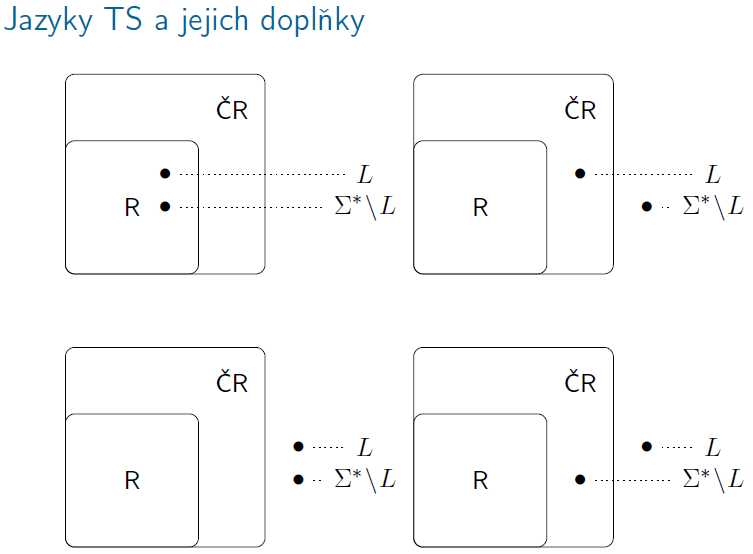
\includegraphics[width=12cm]{img/jazykyAJejichDoplnky.png}
		\caption{Jiné stavy nastat nemůžou !!!}
		\end{figure}

		\vspace{1cm}
		\textbf{Jazyky, které jsou částečně rekurzivní ale nejdou rekurzivní:}

		\begin{itemize}
			\item Univezální jazyl $L_{U}$ definován takto : $$L_{U} = \{ [T,w]| T \text{ je } TS \text{, který přijímá } w\}$$
			\item Jazyk $L_{\text{HALT}}$ definován takto:
						$$L_{\text{HALT}} = \{ [T,w]| T \text{ je } TS \text{, který zastaví pro } w\}$$
			\item Jazyk  $L_{\text{NE}}$ definován takto:
					$$L_{\text{NE}} = \{ [ T ] |  L(T)  \neq  \emptyset\} \text{\dots (zastaví alespoň pro jedno slovo)} $$

		\end{itemize}

		\textbf{Jazyky, které nejsou částečně rekurzivní:}

		\begin{itemize}
			\item Diagonální jazyk $L_{d}$ $$L_{d} = \{[T]| T \text{ je } TS \text{, který nepřijímá svůj kód} \}$$
			\item Jazyk strojů přijímajících prázdný jazyk
				$$L_{\emptyset} = \{[T]| T \text{ je } TS \text{ a } L(T) =
						\emptyset \} \text{\dots(všechny slova zamítne?)}$$
			\item Jazyk strojů, které se nezacyklí
				$$L_{noncycle} = \{ [T]| T \text{ je } TS \text{ a necyklí pro žádné slovo } w\}$$
		\end{itemize}

		\vspace{1cm}
		JAZYK $\approx$ PROBLÉM

		\begin{itemize}
			\item $L_{U} \rightarrow$ problém přijetí
			\item $L_{HALT} \rightarrow$ problém zastavení
			\item $L_{NE} \rightarrow$ problém neprázdnosti jazyka
		\end{itemize}
		\vspace{1cm}


	\subsection{Uzávěrové vlastnosti jazyků TS}

	\textbf{Věty:}
		\begin{itemize}
			\item Pokud $L$ je rekurzivní pak, $\Sigma^{*} \setminus  L$ je rekurzivní (staší sestrojit TS který rozhoduje L
				a prohodit přijímací a zamítací stavy).
			\item Nechť $L_{1}, L_{2} \in R$ jsou rekurzuvní jazyky, pak $L_{1} \cup L_{2} \in R$  a  $L_{1} \cap L_{2} \in R$.
			\item Nechť $L_{1},L_{2} \in R$, pak $L_{1} \circ  L_{2}\in R$
			\item Pokud $L \in R$, pak $L^{*} \in R$ \dots($L^{*}$ je kleenyho uzávěr- zřetězení slov z L)



			\item Nechť $L_{1}, L_{2} \in ČR$ pak:
				\begin{itemize}
					\item $L_{1} \cup L_{2} \in ČR$
					\item $L_{1} \cap L_{2} \in ČR$
					\item $L_{1} \circ L_{2} \in ČR$
					\item $L^{*} \in ČR$
				\end{itemize}
			\item Pokud $L \in ČR$ a  $\Sigma^{*} \setminus  L \in ČR$, pak $L \in R$

		\end{itemize}

	\subsection{Riceova věta :}

	Nechť $L$ je jazyk, jehož slova jsou kódy TS, a platí:
	\begin{itemize}
		\item pokud $L(T_{1}) = L(T_{2})$, pak $[T_{1}] \in L \leftrightarrow [T_{2}] \in L $
		\item $\exists T_{1},T_{2}$ t.ž. $ [T_{1}] \in L, [T_{2}] \notin L$
	\end{itemize}
	pak L není rekurzivní.\\
	\vspace{0,5cm}

	\textit{\textbf{Věta slovně:} Pokud se rovnají jazyky strojů, pak jejich kódydo jazyku buďto oba
				patří nebo oba nepatří a dále existuje alespoň jeden stoj jehož kód do tohoto jazyka nepatří a
				 alespoň jeden který do něj patří, pak není rekurzivní. (zjevně vyplývá třetí podmínka že slova
				 těchto jazyků musí být kódy TS)}\\

	\vspace{0,5cm}

	Tvzdení ve tvaru implikace né ekvilalence! Tzn. že lze použít pouze k důkazu, že nějaký jazyk není rekurzivní a nelze použít
	k důkazu že nějaký jazyk je rekurzivní.


	\subsection{Vztah jazyků TS k jazykům Chomského hierarchie}

		\vspace{5mm}
		$$\text{Typ 3} \subset \text{Typ 2} \subset \text{Typ 1} \subset \text{R} \subset \text{Typ 0} = \text{ČR} $$
		\begin{itemize}
		\item regulární jazyky = jazyky KA
		\item bezkontextové jazyky = jazyky nedeterministických ZA
		\item kontextové jazyky = jazyky LBA
		\item jazyky gen. gramatikami bez omezení = jazyky přijímané TS
		\end{itemize}


		\textbf{Věty: }
		\begin{itemize}
		\item Třídy jazyků generovaných gramatikami typu 0 = částečně rekurzivní jazyky.
		\item Jazyky generované kontextově závislými gramatikamy = jazyky přijímané LBA
		\item Existuje rekurzivní jazyk, který není generovaný kontextovou gramatikou.
		\end{itemize}

		\begin{figure}[!h]
		\centering
		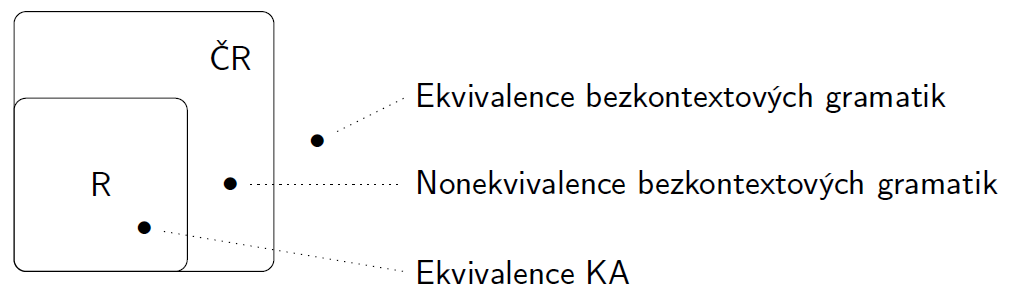
\includegraphics[width=8cm]{img/chomskyVSts.png}
		\end{figure}

	\subsection{Věta o rekurzi}

		TS \textit{vyčísluje funkci $f$}, pokud pro každé slovo $w \in \Sigma^{*}$ zapíše na pásku $f(w)$ a skončí.
		\vspace{5mm}

		\textbf{Věta o rekurzi: }Nechť $T$ je TS, který vyčísluje
			$t : \Sigma^{*} \times \Sigma^{*} \rightarrow \Sigma^{*}$. Existuje TS $R$, který
		počítá funkci $ r : \Sigma^{*} \rightarrow \Sigma^{*}$, kde pro každé $w$ platí $$r(w) = t(\langle R \rangle,w)$$

		\textit{Tvrzení věty říká, že abychom vytvořili TS $R$, který pracuje s vlastním kódem, stačí umět udělat
			 TS $T$, který pracuje stejně, ale dostává kód [R] na vstup. }\\

		\vspace{5mm}
		\textbf{Aplikace věty o rekurzi -- Věta o pevném bodě:}
		Nechť $t : \Sigma^{*} \rightarrow \Sigma^{*}$ je vyčíslitelná funkce. Pak existuje TS $F$, t.ž. $t([F])$ je kód
		ekvivalentního TS.

%============================================================================
%                                                                             TŘETÍ ODSTAVEC
%============================================================================

\section{Třetí odstavec}

Složitost algoritmu (časová a paměťová). Třída P, třída NP, důvody jejich zavedení, jejich vzájemný vztah. NP-
úplné problémy. Cook-Levinova věta. Příklady NP-úplných problémů, dokazovaní NP-úplnosti. Třída PSPACE,
její vztah k třídám P a NP, PSPACE-úplné problémy. Třídy N a NL a NL-úplné problémy.

	\subsection{Složitost algoritmu(časová a paměťová)}

		\textbf{Časová složitost} = funkce $f : N \rightarrow N_{0}$, kde $f(n)$ je maximální
		počet kroků při výpočtu nad jakýmkoli vstupem délky $n$.\\
		\vspace{3mm}

		\textbf{Paměťová složitost} = funkce $f : N \rightarrow N$, kde $f(n)$ je maximální
		 počet kroků při výpočtu nad jakýmkoli vstupem délky $n$.
		\\\vspace{3mm}

		$f,g : N \rightarrow R$\\
		$g(n)$ je \textbf{asymptotická hosní hranice} $f(n)$, když existují $c, n_{0} \in N$, t.ž. pro každé $n~\geq~n_{0}$:
		$$f(n) \leq c \cdot g(n)$$
		Notace: $f(n) = O(g(n))$


	\subsection{Třída P, NP, důvody jejich zavedení, vzájemný vztah}

		\textbf{turingův stroj}
		$$TIME(t(n)) = \{ L | L \text{rozhodovaný TS v čase} O(t(n))\}$$
		$$SPACE(s(n)) = \{ L | L \text{rozhodovaný TS v paměti} O(s(n))\}$$
		\vspace{3mm}
		\textbf{nedeterministický turingův stroj}

		NTS časová složitost t(n) \dots TS časová složitost $2^{O(t(n))}$\\

		NTS paměťová složitost t(n) \dots TS časová složitost $O(t^{2} (n))$

		$$NTIME(t(n)) = \{ L | L \text{rozhodovaný NTS v čase} O(t(n))\}$$
		$$NSPACE(s(n)) = \{ L | L \text{rozhodovaný NTS v paměti} O(s(n))\}$$\\

		\vspace{3mm}
		\textbf{Třídy P a NP:}
		$$P = \bigcup\{TIME(n^k) | k \in N\}$$
		$$NP = \bigcup\{NTIME(n^k) | k \in N\}$$
	\vspace{3mm}

	Víme že $$P\subseteq NP$$

	co ale nevíme je jestli $$NP\subseteq P \text{ tzn. (P=NP) nebo jestli } NP\nsubseteq P$$


	\subsection{NP--úplné problémy}

		Funkce $f :  \Sigma^{*} \rightarrow \Sigma^{*}$ je \textbf{funkce vyčíslitelná v polynomiálním čase}, pokud existuje TS
		pracující v polynomiálním čase, který pro každé $w \in  \Sigma^{*}$ zastaví a na pásce má zapsáno $w$.

		Jazyk A je \textbf{redukovatelný v polynomiálním čase} na jazyk B, načeno $A \leq_P B$, pokud existuje redukce
		v polynomiálním čase, tj. $r :  \Sigma^{*} \rightarrow \Sigma^{*}$, t.ž. $$w \in A \text{ p. k. } f(w) \in B$$

		\vspace{3mm}
		Jazyk B je \textbf{NP-úplný}, pokud
		\begin{itemize}
			\item B je v NP
			\item B je NP-těžký. Tj. pro každý $A\in NP$ platí $A\leq_P B$
		\end{itemize}

		\vspace{3mm}
		\textbf{Věty:}
		\begin{itemize}
			\item Pokud B je NP-úplný a $B \in P$, pak $P = NP$
			\item Pokud B je NP-úplný a $B \leq_P C$ pro $C \in $ NP, pak je NP-úplný
			\item SAT je NP-úplný
			\item 3SAT je NP-úplný
		\end{itemize}

		Hlavní důvod, proč jsou NP-úplné úlohy tak zajímavé, je právě jejich velmi obtížná řešitelnost. Díky ní nacházejí uplatnění v
 		moderní kryptografii, kde musíme být schopni rychle ověřovat správnost řešení, ale jeho nalezení musí trvat dlouho. Obtížnost
		výpočtu ovšem záleží i na konkrétních datech, pro speciální množinu vstupů může být úloha polynomiální, například řešíme-li
		obarvení třemi barvami pro jednoduché grafy (cesty).



	\subsection{Cook--Levinova věta}
		\textbf{Věta:} SAT je NP-úplný \dots (vic k tomu nemáme a důkaz psat nebudu stejně byste
			 se na to vysrali a mě už ten \LaTeX  pěkně mrdá)

	\subsection{Příklady NP--úplných problémů}
		\begin{itemize}
			\item SAT je NP-úplný
			\item 3SAT je NP-úplný
			\item  hledání  hamiltonovské kružnice v grafu
			\item vrcholové pokrytí
			\item trojrozměrné párování
		\end{itemize}

	\subsection{Dokazování NP--úplnosti}

		\textbf{Věta:} Pokud B je NP-úplný a $B \leq_P C$ pro $C \in $ NP, pak $C$ je NP-úplný

	\subsection{Třída PSPACE, její vztah k třídám P a NP}

		PSPACE je třída jazyku, které jsou rozhodnutelné v polynomickém čase na (deterministickém) TS, tedy
		$$\text{PSPACE} = \bigcup_k \text{SPACE}(n^k)$$
		Ze Savitchovy věty plyne že $$\text{PSPACE} = \text{NPSPACE}$$
		Celkově tedy máme:
		$$\text{ P } \subseteq \text{ NP } \subseteq \text{ PSPACE } \subseteq \text{ EXPTIME } $$  kde
		$\text{EXPTIME} = \bigcup_k \text{TIME}(2^n)$\\
		Alespoň jedna z těchto inkluzí je vlastní: ví se, že P~$\neq$~EXPTIME.\\
		Věří se, že všechny ty jsou vlastní.


	\subsection{PSPACE--úplné problémy}

		Jazyk $B$ je \textbf{PSPACE-úplný problém}, pokud
		\begin{itemize}
			\item $B \in$ PSPACE
			\item $B$ je PSPACE-těžký, tj. každý $A \in$ PSPACE he redukovatelný v polynomickém čase na $B$
		\end{itemize}\vspace{3mm}
		\textbf{Grafová hra:} Mějme orientovaný graf G s vyznačeným počátečním uzlem $u_1$
		\begin{itemize}
			\item Aktuální uzel je na začátku $u_1$
			\item Hráči se střídají v tazích
			\item Hráč na tahu zvolí souseda $u_1$, ten se stává aktuálním uzlem, nelze vybrat uzel, který už byl předtím
				navštíven
			\item Hráč, který uvízne prohrává
		\end{itemize}
		$$GG = \{[G,b] | \text{ hráč 1 má vítěznou strategii pro G a poč. b } \}$$\\

		GG je PSPACE-úplný.



	\subsection{Třídy L, NL a NL--úplné problémy}

		$$\text{L = SPACE}(log(n))$$
		$$\text{NL = NSPACE}(log(n))$$

	Omezujeme se na logaritmickou paměťovou složitost ze stejného důvodu, jako jsme se předtím omezili na
	 polynomickou časovou složitost: problémy řešitelné v logaritmické paměti považujeme za řešitelné efektivně.

		\begin{figure}[!h]
		\centering
		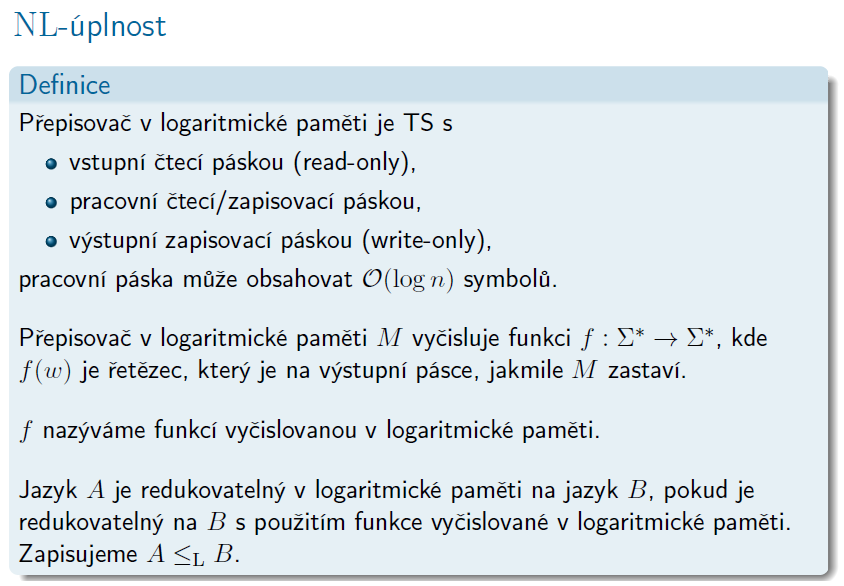
\includegraphics[width=13cm]{img/prepisovac.png}
		\end{figure}

		\begin{figure}[!h]
		\centering
		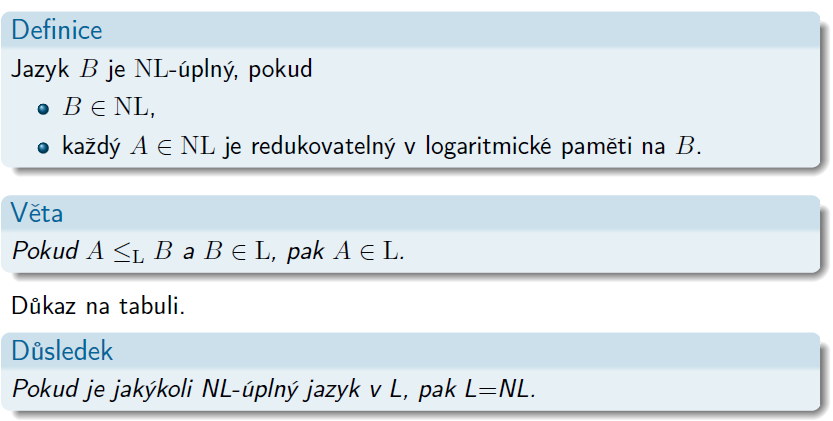
\includegraphics[width=13cm]{img/NLuplny.png}
		\end{figure}


%============================================================================
%                                                                            ČTVRTÝ ODSTAVEC
%============================================================================

\section{Čtvrtý odstavec}

Výroková logika: jazyk, formule, pravdivostní ohodnocení, tautologie, tabulková metoda, sémantické vyplývání,
normální formy formulí, úplné systémy spojek. Axiomatický systém výrokové logiky, syntaktické vyplývání. Věta
o dedukci. Věty o korektnosti a úplnosti výrokové logiky. Predikátová logika: jazyk, termy a formule, struktury
pro jazyk, ohodnocení termů a formulí. Axiomatický systém predikátové logiky, syntaktické vyplývání. Věty o
korektnosti a úplnosti predikátové logiky. Neklasické logiky, fuzzy logika. Základy logického programování, úvod
do Prologu.


	\subsection{Výroková Logika}

		\subsubsection{jazyk}
			\begin{figure}[!h]
			\centering
			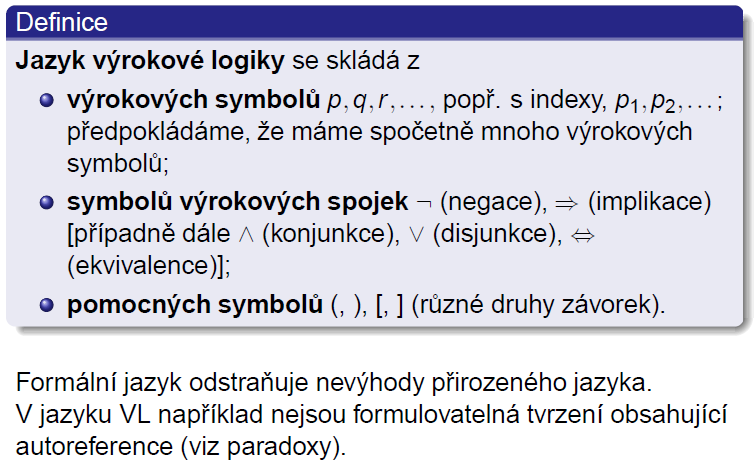
\includegraphics[width=13cm]{img/jazykVL.png}
			\end{figure}

			\begin{figure}[!h]
			\centering
			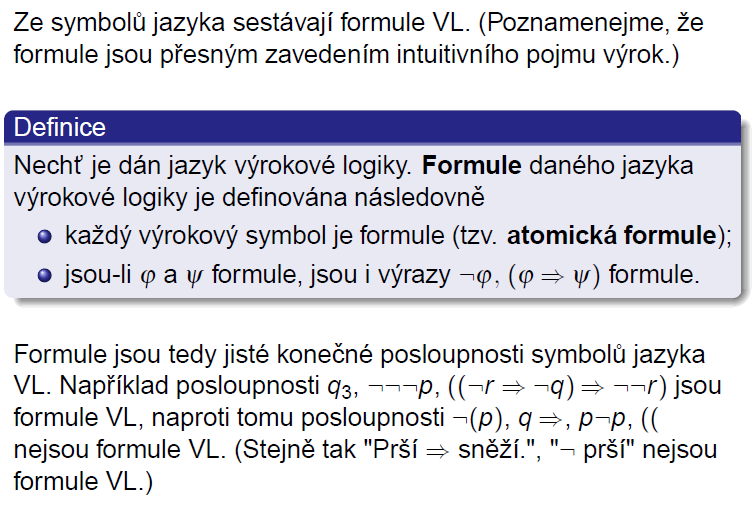
\includegraphics[width=13cm]{img/formuleVL.png}
			\end{figure}
 		\newpage
		\subsubsection{pravdivostní ohodnocení}

			\begin{figure}[!h]
			\centering
			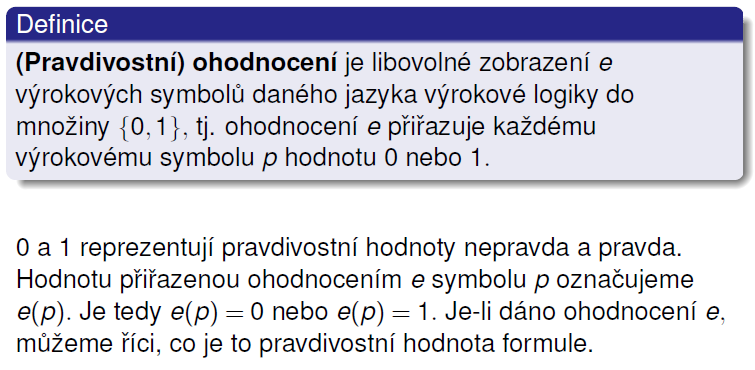
\includegraphics[width=13cm]{img/pravdivostniOhodnoceniVL.png}
			\end{figure}

			\begin{figure}[!h]
			\centering
			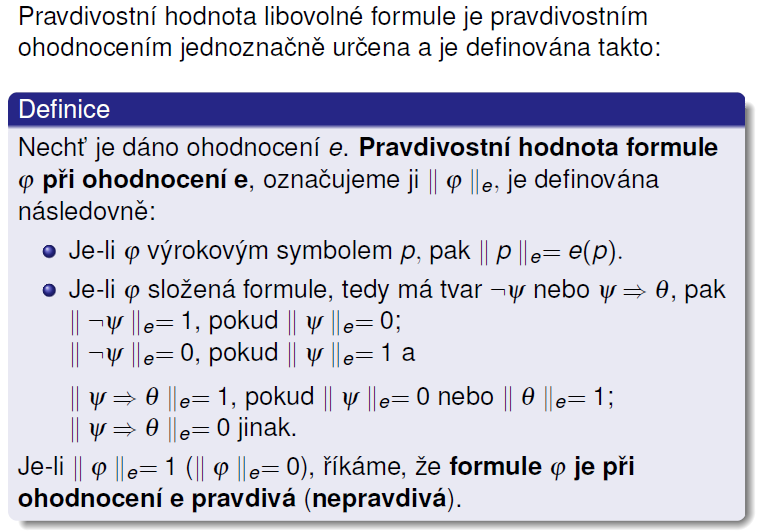
\includegraphics[width=13cm]{img/ohodnoceniFormule.png}
			\end{figure}

		\newpage
		\subsubsection{tautologie}

		\begin{figure}[!h]
			\centering
			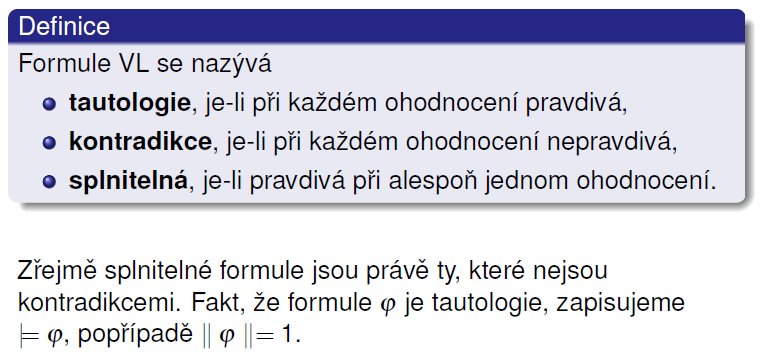
\includegraphics[width=13cm]{img/tautologie.png}
			\end{figure}

		\subsubsection{tabulková metoda}
			\begin{figure}[!h]
			\centering
			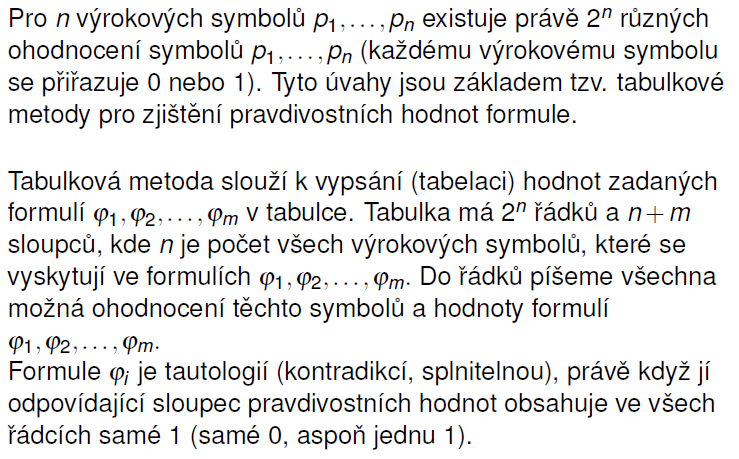
\includegraphics[width=13cm]{img/tabulkovaMetoda.png}
			\end{figure}

		\newpage
		\subsubsection{sémantické vyplývání}

			\begin{figure}[!h]
			\centering
			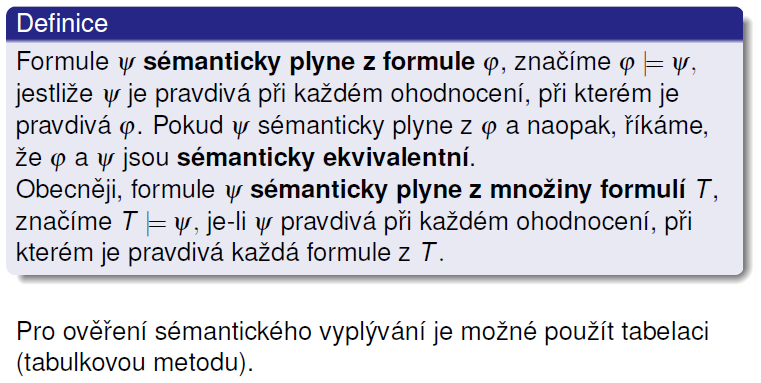
\includegraphics[width=13cm]{img/semantickeVyplyvani.png}
			\end{figure}

		\subsubsection{normální formy formulí}

			\begin{figure}[!h]
			\centering
			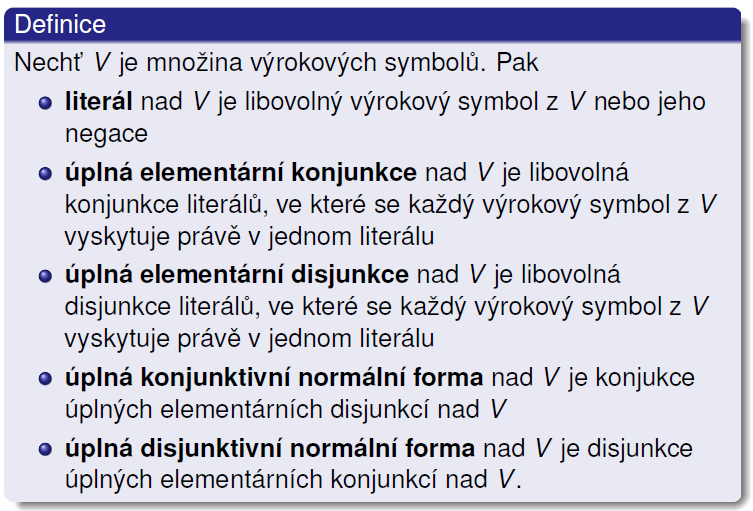
\includegraphics[width=13cm]{img/UKNF.png}
			\end{figure}

			\begin{figure}[!h]
			\centering
			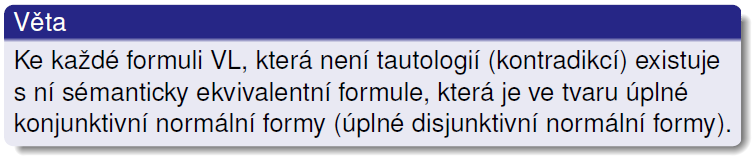
\includegraphics[width=13cm]{img/vetaUKNF.png}
			\end{figure}

			\begin{figure}[!h]
			\centering
			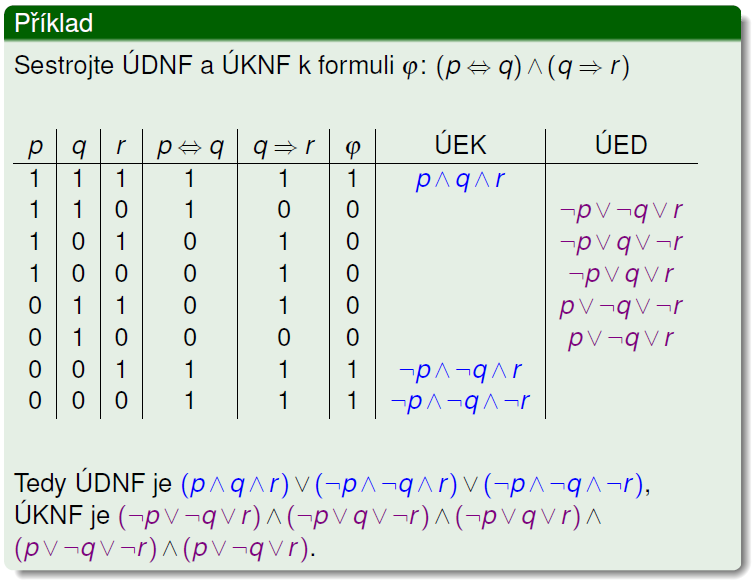
\includegraphics[width=13cm]{img/prikladUKNF.png}
			\end{figure}


		\subsubsection{úplné systémy spojek}

			\begin{figure}[H]
			\centering
			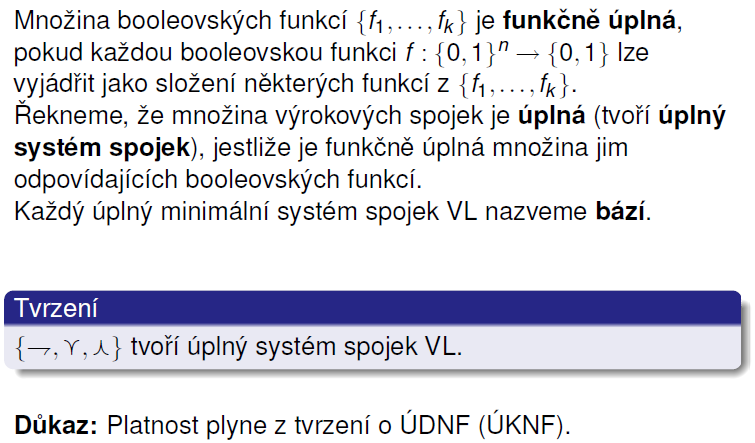
\includegraphics[width=13cm]{img/uplneSystemySpojek.png}
			\end{figure}

			\begin{figure}[H]
			\centering
			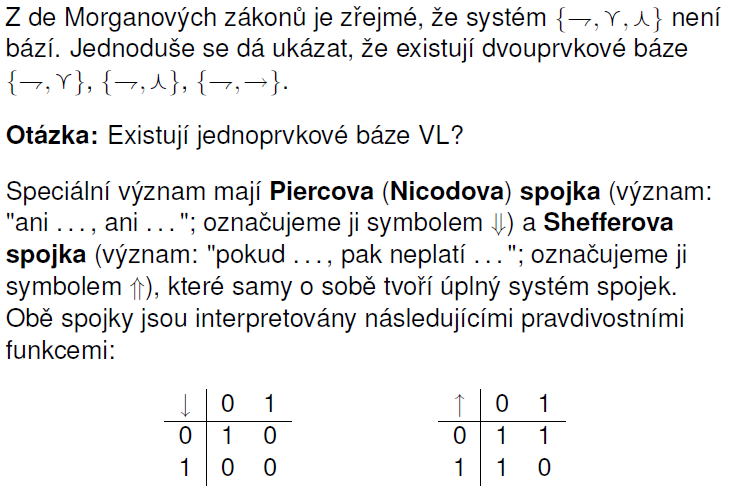
\includegraphics[width=13cm]{img/uplneSystemySpojek2.png}
			\end{figure}

			Existují pouze 2 jednoprvkové báze (Sheffer a Nicod)

		\subsubsection{axiomatický systém výrokové logiky}

			\begin{figure}[H]
			\centering
			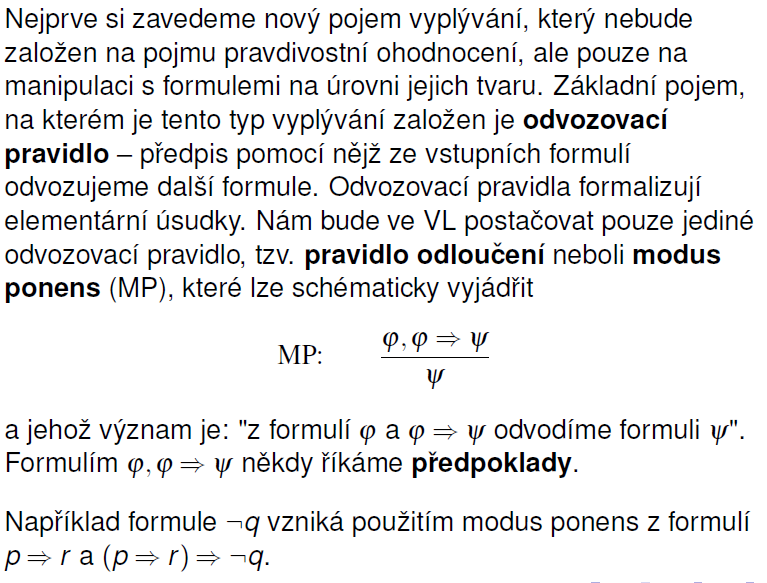
\includegraphics[width=12cm]{img/MP.png}
			\end{figure}

			\begin{figure}[H]
			\centering
			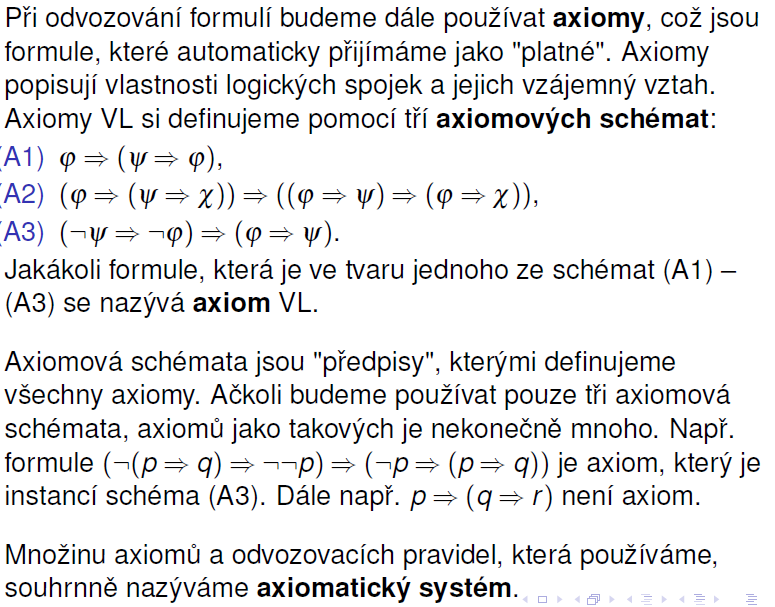
\includegraphics[width=12cm]{img/axiomy.png}
			\end{figure}

		\subsubsection{syntaktické výplývání}

			\begin{figure}[H]
			\centering
			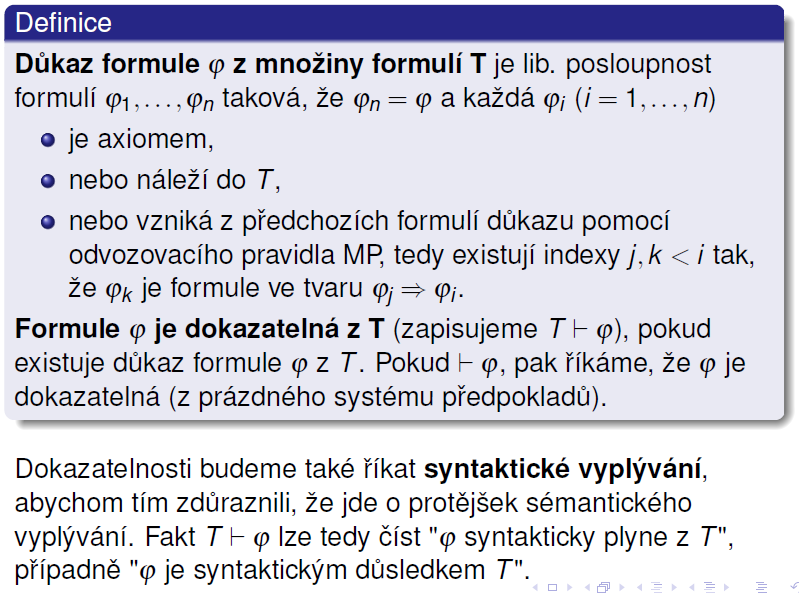
\includegraphics[width=12cm]{img/dukaz.png}
			\end{figure}

		\subsubsection{Věta o dedukci}

			\begin{figure}[H]
			\centering
			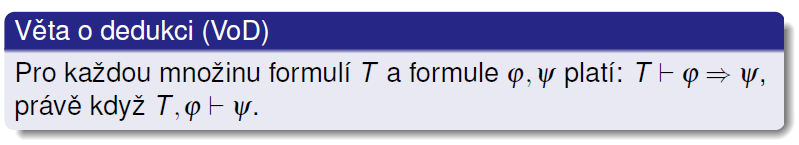
\includegraphics[width=13cm]{img/VoD.png}
			\end{figure}

			\begin{figure}[H]
			\centering
			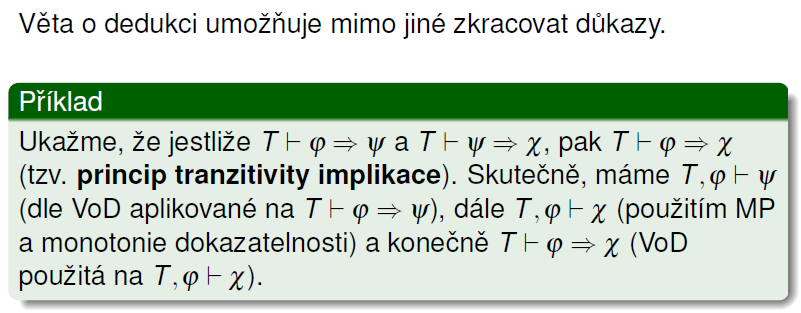
\includegraphics[width=13cm]{img/VoDpriklad.png}
			\end{figure}

		\subsubsection{Věty o korektnosti a úplnosti výrokové logiky}

			\begin{figure}[H]
			\centering
			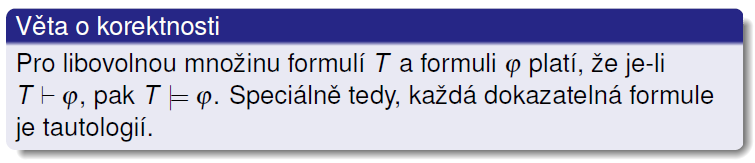
\includegraphics[width=13cm]{img/VoK.png}
			\end{figure}

			\begin{figure}[H]
			\centering
			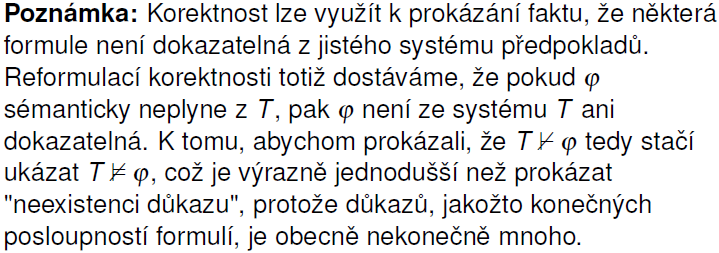
\includegraphics[width=13cm]{img/VoKpoznamka.png}
			\end{figure}

			\begin{figure}[H]
			\centering
			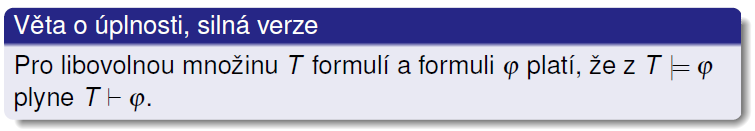
\includegraphics[width=13cm]{img/VoU.png}
			\end{figure}

	\subsection{Predikátová logika}

		\subsubsection{jazyk}

			\begin{figure}[H]
			\centering
			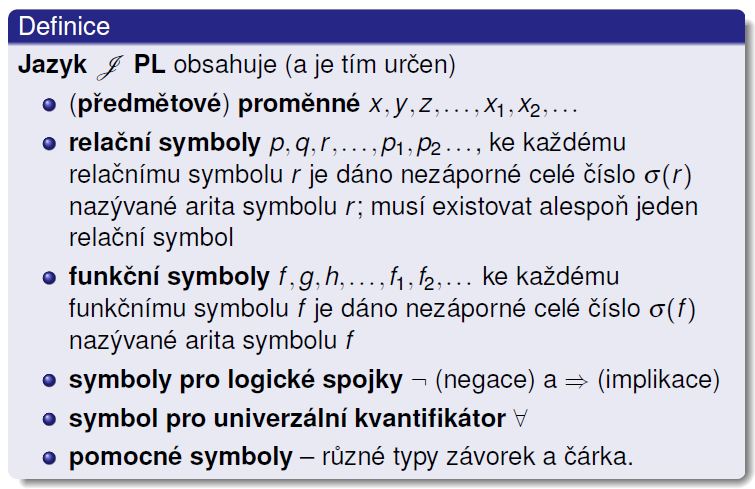
\includegraphics[width=13cm]{img/JazykPL.png}
			\end{figure}

			\begin{figure}[H]
			\centering
			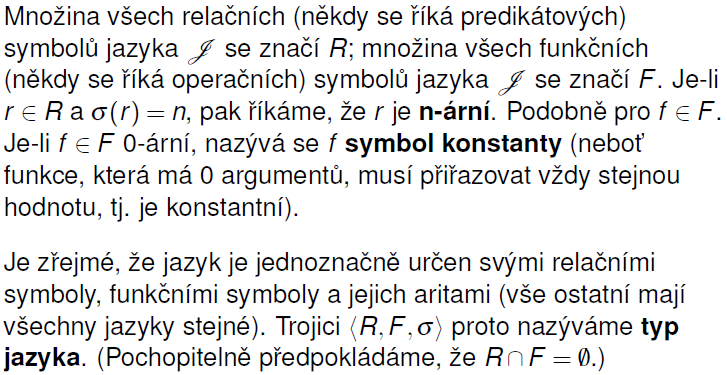
\includegraphics[width=13cm]{img/JazykPL2.png}
			\end{figure}

		\subsubsection{termy a formule}

			\begin{figure}[H]
			\centering
			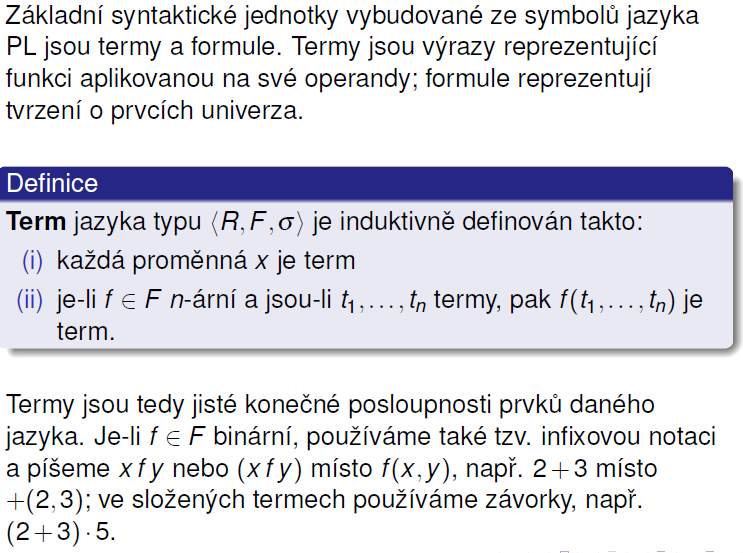
\includegraphics[width=13cm]{img/termy.png}
			\end{figure}

			\begin{figure}[H]
			\centering
			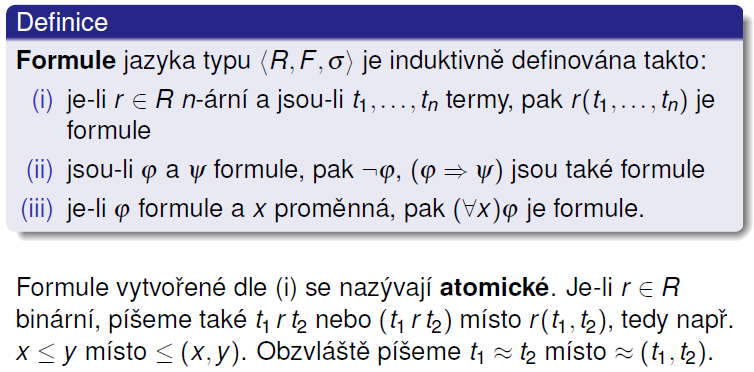
\includegraphics[width=13cm]{img/formulePL.png}
			\end{figure}

		\subsubsection{struktury pro jazyk}

			\begin{figure}[H]
			\centering
			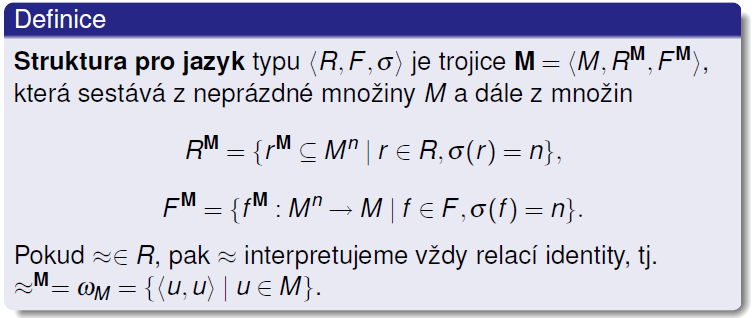
\includegraphics[width=13cm]{img/stukturaProJazyk.png}
			\end{figure}

			\begin{figure}[H]
			\centering
			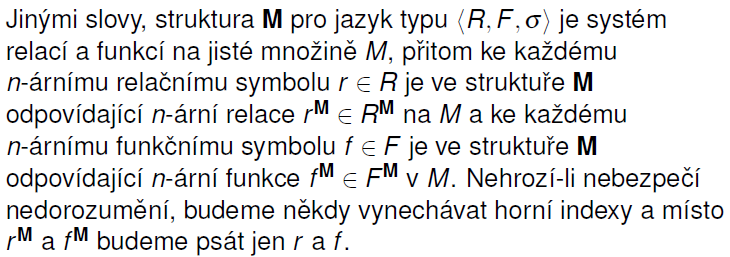
\includegraphics[width=13cm]{img/strukturaProJazyk.png}
			\end{figure}

		\subsubsection{ohodnocení termu a formulí}

			\begin{figure}[H]
			\centering
			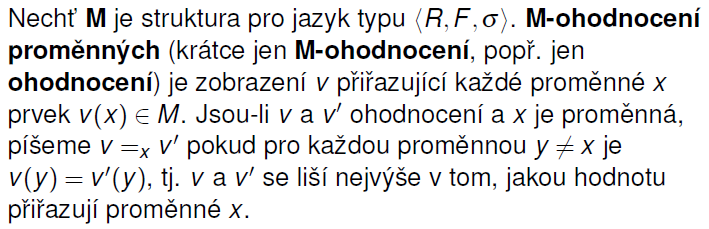
\includegraphics[width=13cm]{img/ohodnoceniPL.png}
			\end{figure}

			\begin{figure}[H]
			\centering
			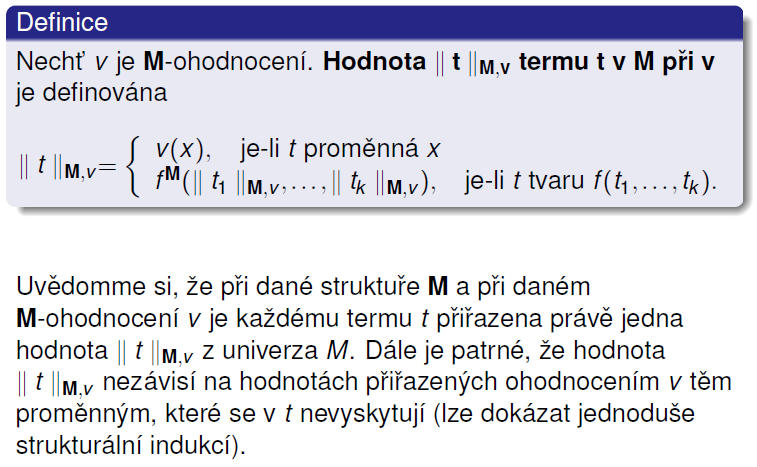
\includegraphics[width=13cm]{img/mOhodnoceni.png}
			\end{figure}

			\begin{figure}[H]
			\centering
			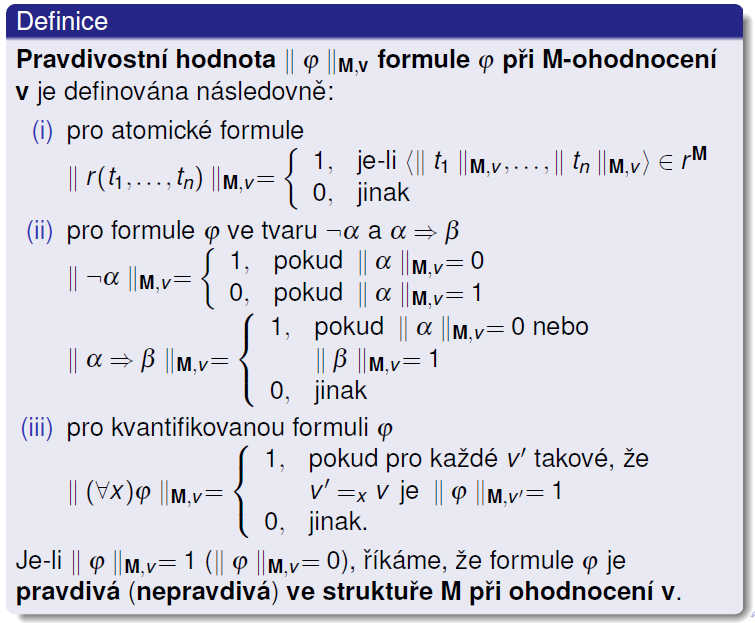
\includegraphics[width=13cm]{img/ohodnoceniFormuliPL.png}
			\end{figure}

		\subsubsection{axiomatický systém predikátové logiky}

			\begin{figure}[H]
			\centering
			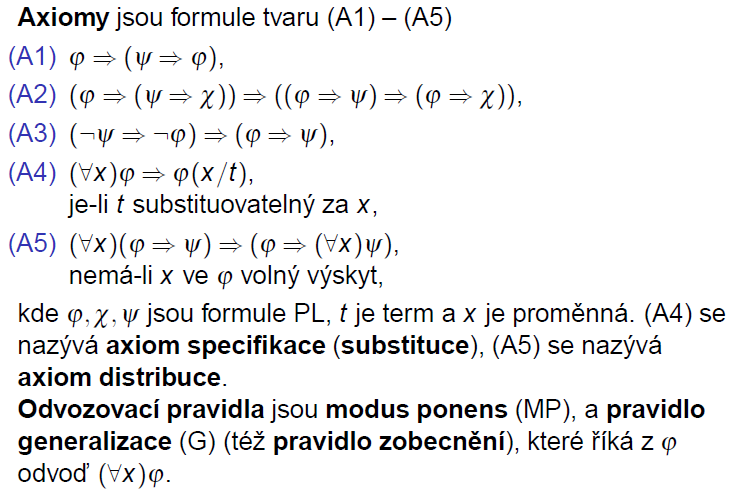
\includegraphics[width=13cm]{img/axiomyPL.png}
			\end{figure}

		\subsubsection{syntaktické vyplývání}

			\begin{figure}[H]
			\centering
			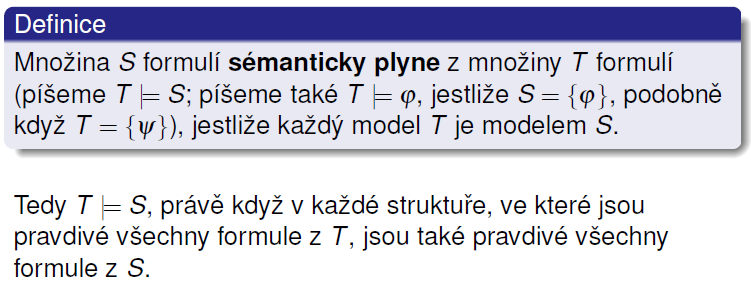
\includegraphics[width=13cm]{img/semantickeVyplyvaniPL.png}
			\end{figure}

			\begin{figure}[H]
			\centering
			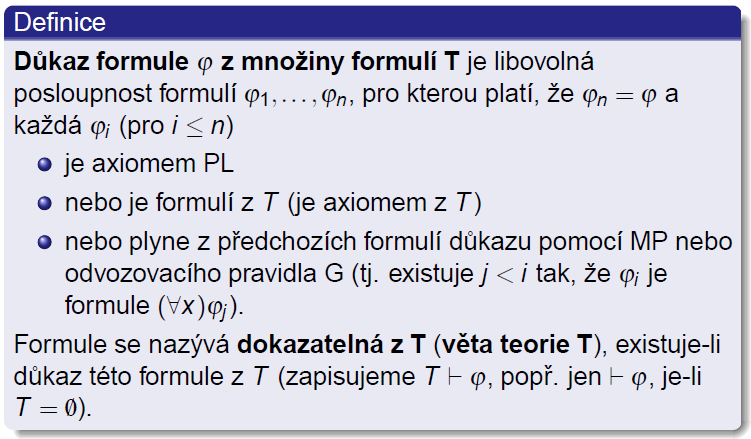
\includegraphics[width=13cm]{img/syntaktickeVyplyvaniPL.png}
			\end{figure}

			Formule je dokazatelná z T = formule syntakticky plyne z T.


		\subsubsection{věty o korektnosti a úplnosti predikátové logiky}

			\begin{figure}[H]
			\centering
			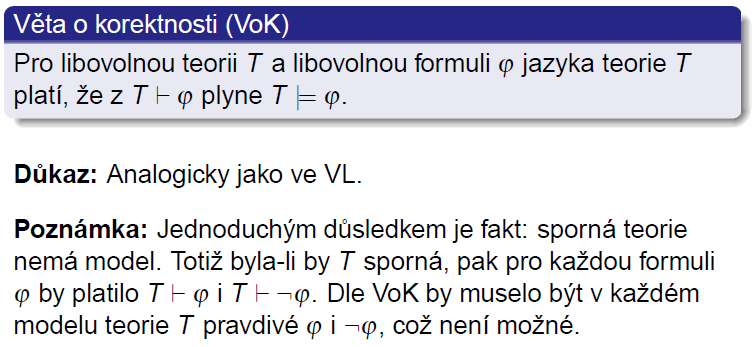
\includegraphics[width=13cm]{img/VoKPL.png}
			\end{figure}

			\begin{figure}[H]
			\centering
			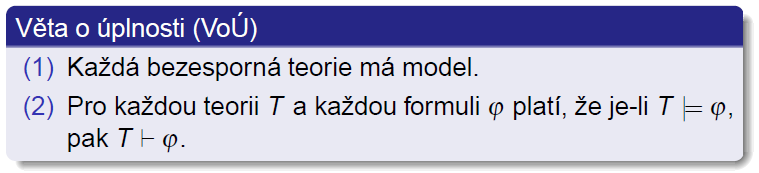
\includegraphics[width=13cm]{img/VoUPL.png}
			\end{figure}

	\subsection{Neklasické logiky}
		\begin{itemize}
			\item Modální logika (založena na pojmu \uv{možný svět}, spojky:\textit{ je možné že, je nutné že})
			\item Temporální logika (logika času - pravdivost tvrzení závisí na čase)
			\item Epistemická logika (logika znalostí, spojky: \textit{ví se že, věří se že})
			\item Fuzzy logika
		\end{itemize}

		\subsubsection{fuzzy logika}

			\begin{figure}[H]
			\centering
			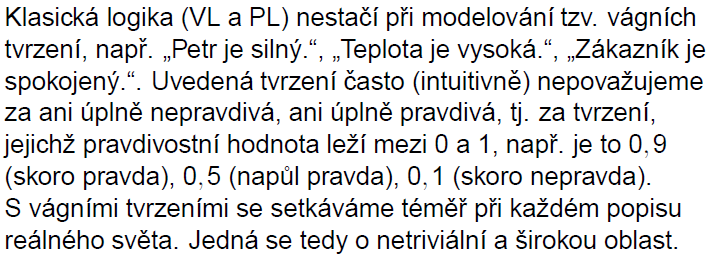
\includegraphics[width=13cm]{img/fuzzy1.png}
			\end{figure}

			\begin{figure}[H]
			\centering
			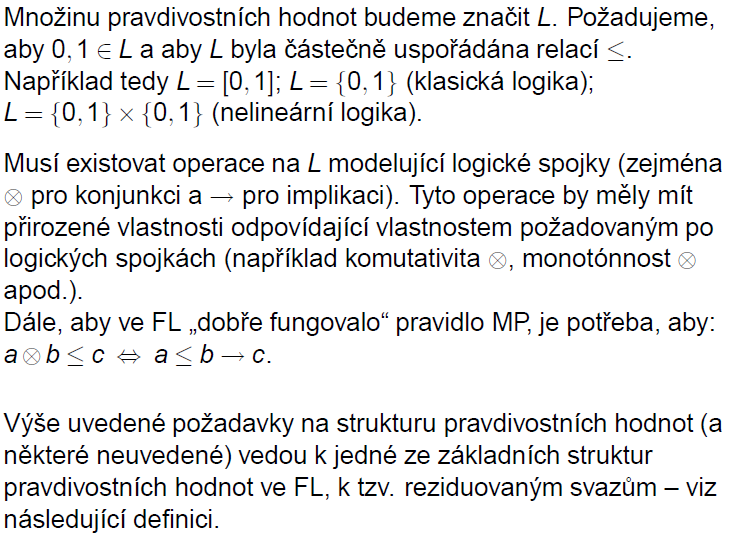
\includegraphics[width=13cm]{img/fuzzy2.png}
			\end{figure}

			\begin{figure}[H]
			\centering
			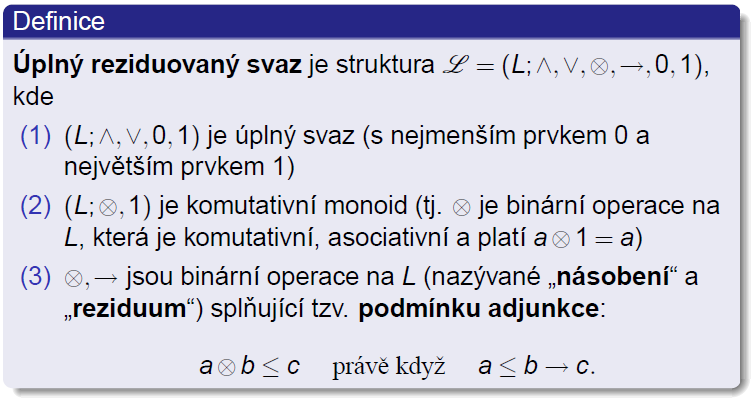
\includegraphics[width=13cm]{img/fuzzy3.png}
			\end{figure}

			\begin{figure}[H]
			\centering
			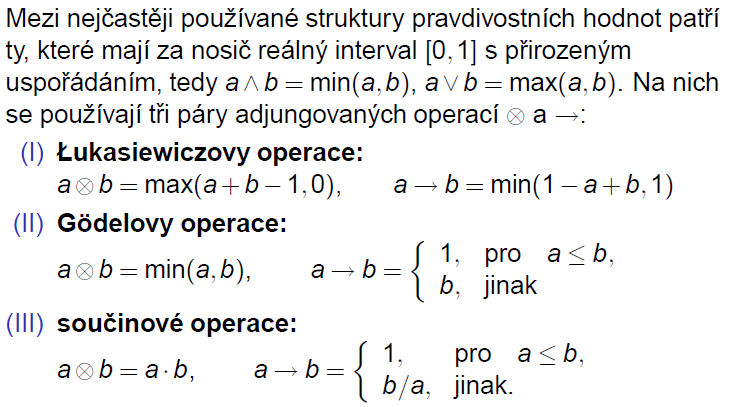
\includegraphics[width=13cm]{img/fuzzy4.png}
			\end{figure}


	\subsection{Základy logického programování, úvod do Prologu}

			\begin{figure}[H]
			\centering
			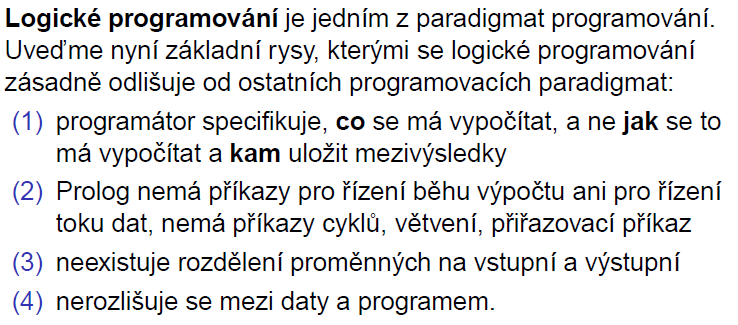
\includegraphics[width=13cm]{img/prolog1.png}
			\end{figure}

			\begin{figure}[H]
			\centering
			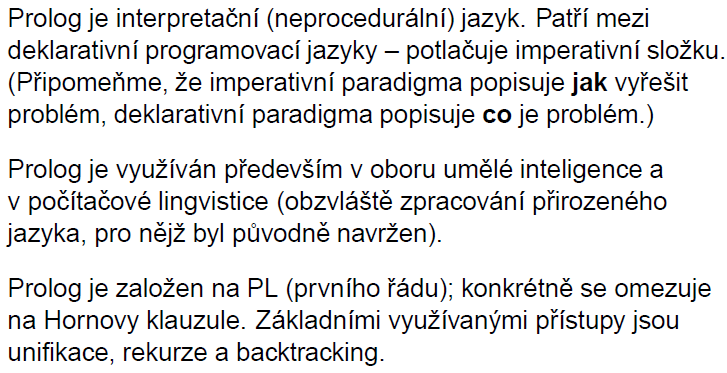
\includegraphics[width=13cm]{img/prolog2.png}
			\end{figure}

			\begin{figure}[H]
			\centering
			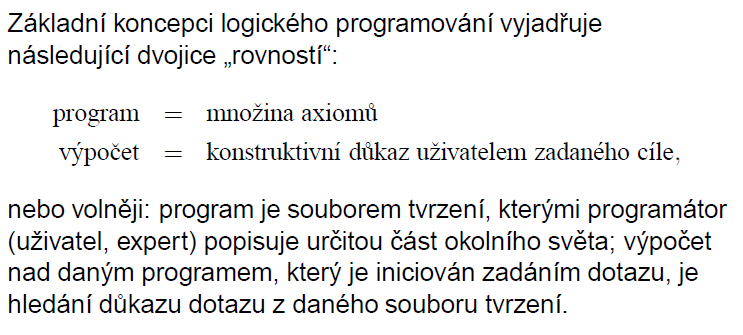
\includegraphics[width=13cm]{img/prolog3.png}
			\end{figure}

			\begin{figure}[H]
			\centering
			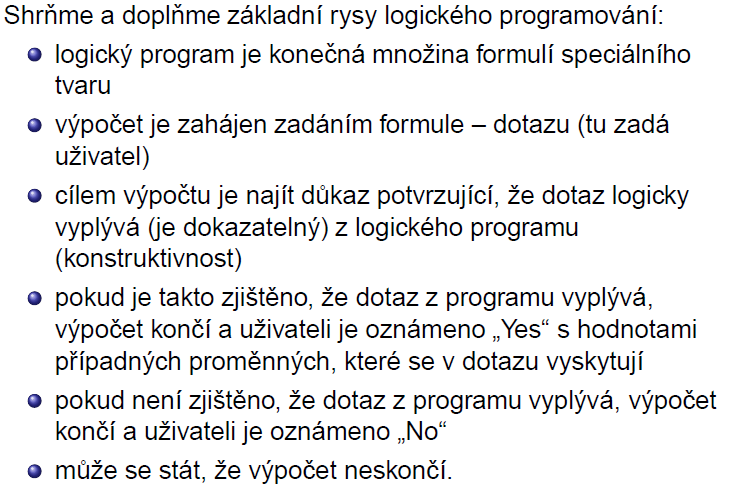
\includegraphics[width=13cm]{img/prolog4.png}
			\end{figure}

			\begin{figure}[H]
			\centering
			
\includegraphics[width=13cm]{img/prolog5.png}
			\end{figure}

			\begin{figure}[H]
			\centering
			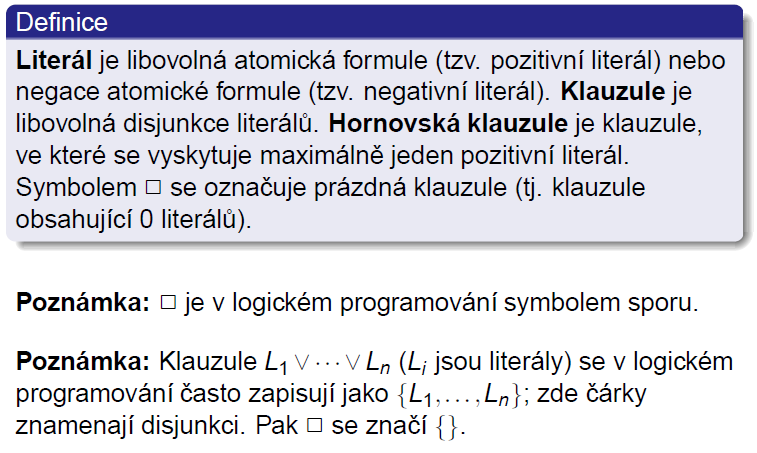
\includegraphics[width=13cm]{img/prolog6.png}
			\end{figure}

			\begin{figure}[H]
			\centering
			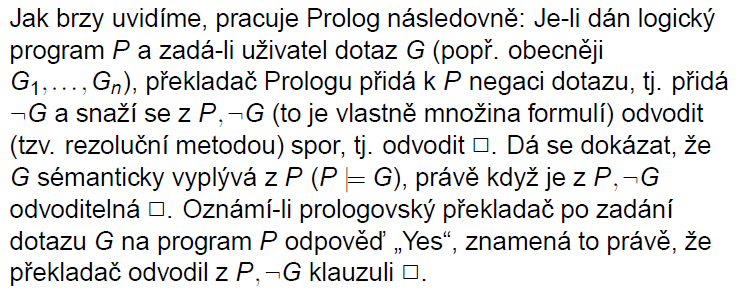
\includegraphics[width=13cm]{img/prolog7.png}
			\end{figure}

			\begin{figure}[H]
			\centering
			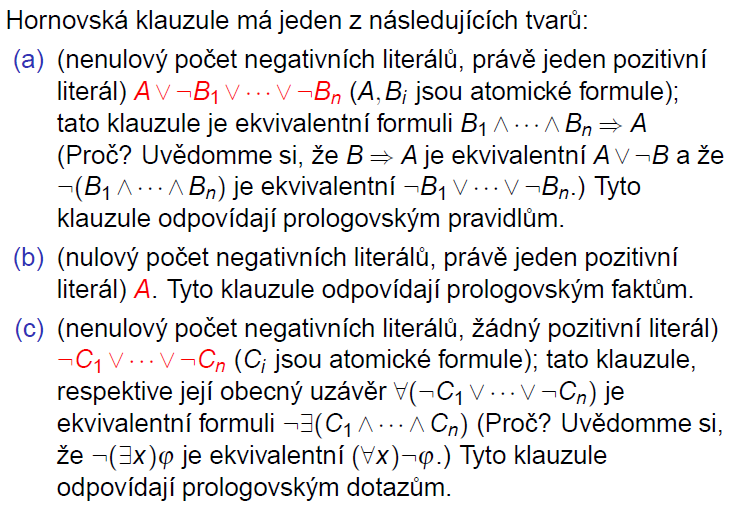
\includegraphics[width=13cm]{img/prolog8.png}
			\end{figure}

			\begin{figure}[H]
			\centering
			\includegraphics[width=13cm]{img/prolog9.png}
			\end{figure}

	Zbytek prologu už je nechutně hnusnej a radši chcípnu než abych se to zas učil.


\end{document}
